
\documentclass[a4paper,UKenglish,cleveref, autoref, thm-restate]{lipics-v2021}
\nolinenumbers
\bibliographystyle{plainurl}% the mandatory bibstyle


\newcommand{\UB}{\text{UB}}
\newcommand{\LB}{\text{LB}}

\usepackage[linesnumbered,ruled,vlined]{algorithm2e}
\SetKw{Or}{or}
\SetKw{Not}{not}

\usepackage[dvipsnames]{xcolor}

\usepackage{tikz}
\usetikzlibrary{decorations.pathreplacing,calligraphy}


\title{SAT-based Leximax Optimisation Algorithms} 



\author{Miguel Cabral}{INESC-ID, IST - Universidade de Lisboa, Portugal}{miguel.cabral@tecnico.ulisboa.pt}{}{}
\author{Mikol\'a\v s Janota}{Czech Technical University Prague, Czechia}{mikolas.janota@gmail.com}{https://orcid.org/0000-0003-3487-784X}{}
\author{Vasco Manquinho}{INESC-ID, IST - Universidade de Lisboa, Portugal}{vasco.manquinho@tecnico.ulisboa.pt}{https://orcid.org/0000-0002-4205-2189}{}

\authorrunning{M. Cabral, M. Janota and V. Manquinho} 

\Copyright{Miguel Cabral, Mikol\'a\v s Janota and Vasco Manquinho} 

\ccsdesc[500]{Computing methodologies~Optimization algorithms}


\keywords{Multi-Objective Optimisation, Leximax, Sorting Networks} 

\category{} 

\relatedversion{} 



\acknowledgements{This work was partially supported by Portuguese national funds through FCT, under projects UIDB/50021/2020, PTDC\-/CCI-COM/\-31198/\-2017, PTDC/\-CCI-COM/\-32378/\-2017 and DSAIPA/AI/0044/2018.
%
The results were supported by the Ministry of Education, Youth and Sports
within the dedicated program ERC~CZ under the project \emph{POSTMAN}
no.~LL1902. This article is part of the \emph{RICAIP} project that has received
funding from the European Union's Horizon~2020 research and innovation
programme under grant agreement No~857306. }





\EventEditors{Kuldeep S. Meel and Ofer Strichman}
\EventNoEds{2}
\EventLongTitle{25th International Conference on Theory and Applications of Satisfiability Testing (SAT 2022)}
\EventShortTitle{SAT 2022}
\EventAcronym{SAT}
\EventYear{2022}
\EventDate{August 2--5, 2022}
\EventLocation{Haifa, Israel}
\EventLogo{}
\SeriesVolume{236}
\ArticleNo{29}


\begin{document}

\maketitle

\begin{abstract}
In several real-world problems, it is often the case that the goal is to optimise several objective functions. However, usually there is not a single optimal objective vector.
Instead, there are many optimal objective vectors known as Pareto-optima.
Finding all Pareto-optima is computationally expensive and the number of Pareto-optima can be too large for a user to analyse. 
A compromise can be made by defining an optimisation criterion that integrates all objective functions.

In this paper we propose several SAT-based algorithms to
solve multi-objective optimisation problems using the leximax criterion.
The leximax criterion is used to obtain a Pareto-optimal solution with a 
small trade-off between the objective functions, which is suitable in 
problems where there is an absence of priorities between the objective functions.
Experimental results on the Multi-Objective Package Upgradeability Optimisation problem show that the SAT-based algorithms are able to outperform the Integer Linear Programming (ILP) approach when using non-commercial ILP solvers.
Additionally, experimental results on selected instances from the MaxSAT evaluation adapted to the multi-objective domain show that our approach outperforms the ILP approach using commercial solvers.
\end{abstract}

\section{Introduction}
\label{sec:intro}

In many real-world problems such as Virtual Machine Consolidation~\cite{DBLP:journals/fgcs/LiZLY20}, trip planning~\cite{DBLP:journals/eswa/MarquesRR19},
automated program repair~\cite{DBLP:journals/tse/YuanB20} or Package Upgradeability~\cite{DBLP:journals/jsat/JanotaLMM12}, there
are several objective functions to minimise. 
The challenge with having more than one objective function is that the objective functions may be conflicting. Decreasing one objective function may lead to an increase of another objective function. 
Despite this trade-off, it is possible to discard feasible solutions for which there exists another feasible solution that is able to decrease all objective functions at the same time.
For example, suppose we have two objective functions $f_1$ and $f_2$ and two feasible solutions $\alpha$, $\alpha'$ with objective vectors $(f_1(\alpha),f_2(\alpha))=(10,10)$ and $(f_1(\alpha'),f_2(\alpha'))=(20,20)$. In this case there is no trade-off and $\alpha$ is clearly preferred over $\alpha'$.
This motivates the well-known notion of Pareto-optimality. A Pareto-optimal solution is such that there does not exist another feasible solution that decreases all objective functions at the same time.

When solving a Multi-Objective Boolean Optimisation problem, one can try to enumerate or approximate the set of Pareto-optima (also known as Pareto frontier) and leave it to an expert to choose one of those solutions. The expert does not have to analyse all Pareto-optima, since there are criteria to select a representative subset of Pareto-optimal solutions~\cite{DBLP:journals/cor/GuerreiroMF21}.
A different approach is to transform the multi-objective problem into a single-objective one by using a linear combination of the objective functions. However, defining the weight for each objective function is often unclear for users.

One can also compute a Pareto-optimal solution that is minimal according to a certain order. For example, in the lexicographic order~\cite{BolLexiMarques-Silva2011}, users define priorities to the objective functions. In this case, an optimal solution corresponds to minimising the highest priority objective function, then the second highest priority objective function, and so on.
For instance, the vector $(20,50)$ is lexicographically smaller than the vector $(40, 30)$, assuming an order of priorities from left to right.
However, defining a lexicographic order corresponds to selecting one feasible solution from
the extremes of the Pareto frontier. As a result, the lexicographic-optimum will likely be very unbalanced, i.e.\ some objective functions will have very small values and other objective functions will have very large values. 

Unlike the lexicographic order, the leximax relation tends to provide a small trade-off between the several objective functions. Moreover, the leximax relation does not require the user to predefine an order of priority between the objective functions.
Hence, computing a leximax-optimal solution is suitable in problems where there is an absence of priorities between the objective functions.
In practice, the leximax-optimum corresponds to minimising the maximum value among all objective functions, then the second maximum of the objective functions, and so on.
Therefore, besides minimising the worst value among all objective functions, the solution found using the leximax criterion is usually balanced. Thus, leximax is a natural criterion for solving problems where an order among the objective functions is not defined, returning a balanced solution with good performance.
Finally, observe that the lexicographic-optimum and the leximax-optimum are both a Pareto-optimum~\cite{ehrgott}.

In this paper, we propose several SAT-based leximax optimisation algorithms.
The main contributions of our work are:
\begin{enumerate}
\item new incremental SAT-UNSAT and UNSAT-SAT leximax optimisation algorithms,
\item the use of unsatisfiable cores to improve the performance of UNSAT-SAT
leximax optimisation algorithms,
\item dynamical construction of the CNF representation of the 
objective functions, and
\item an extensive empirical evaluation of our algorithms on the Multi-Objective Package Upgradeability Optimisation problem~\cite{mancoosi-competition} and on randomly generated multi-objective instances based on the MaxSAT Evaluation 2021 benchmarks~\cite{maxsat-eval-2021}.
\end{enumerate}

This paper is organised as follows. In Section~\ref{sec:backg} we formally
define the Multi-Objective Boolean Optimisation problem using the leximax criterion and highlight related work in Multi-Objective Boolean Optimisation 
and leximax optimisation.
Section~\ref{sec:algorithms} describes the new SAT-based leximax optimisation algorithms.
In Section~\ref{sec:evaluation} we evaluate our leximax optimisation algorithms against other state of the art leximax optimisation algorithms.
Finally, Section~\ref{sec:concl} summarises the main contribution of our work. 
\section{Background}
\label{sec:backg}

This paper assumes the standard definitions and notation of propositional logic, including the notions of Boolean variable, literal, clause, conjunctive normal form (CNF) and the Boolean satisfiability (SAT) problem~\cite{handbook}.
Given a set of $m$ literals $l_1, \dots, l_m$ and respective coefficients
$\omega_1, \dots, \omega_m \in \mathbb{N}$, a Pseudo-Boolean (PB) 
expression is a weighted sum of literals $\sum_{i = 1}^m \omega_i \cdot l_i$.
Given an integer $k \in \mathbb{N}$, a linear PB constraint has the form
$\sum_{i = 1}^m \omega_i \cdot l_i \bowtie k, \quad \bowtie \;\in \lbrace \le, \ge, = \rbrace$.

\begin{definition}[Multi-Objective Boolean Optimisation problem (MOBO)]
An instance of MOBO is defined by a vector $f(X) = (f_1(X), \dots, f_n(X))$ of $n$ PB expressions and a
set of PB constraints defined over a set $X$ of Boolean variables.
We assume, without loss of generality, that each objective function is a 
weighted sum of Boolean variables, with positive weights.
\end{definition}

\begin{definition}[Objective vector]
Let $\alpha: X \rightarrow \lbrace 0, 1 \rbrace$ be a complete assignment that 
satisfies all PB constraints in a Multi-Objective Boolean Optimisation instance.
Given an assignment $\alpha$ and objective functions $f = (f_1, \dots, f_n)$, the vector $\vec{f}(\alpha)=(f_1(\alpha),\dots,f_n(\alpha))$ is called the objective vector where $f_i(\alpha)$ is the value of function $f_i$ considering the
assignment $\alpha$.
\end{definition}

\begin{definition}[Pareto-optimal]
Let $\vec{a}=(a_1,\dots,a_n)\in \mathbb{N}^n$ and $\vec{b}=(b_1,\dots,b_n)\in \mathbb{N}^n$. We write $\vec{a} \prec_{\text{Par}} \vec{b}$, if for all $i \in \{1,\dots,k\}$, $a_i\leq b_i$ and there exists $j\in \{1,\dots,k\}$ such that $a_j < b_j$. A feasible solution $\alpha$ is Pareto-optimal if there does not exist another feasible solution $\alpha'$ such that $\vec{f}(\alpha') \prec_{\text{Par}} \vec{f}(\alpha)$.
\end{definition}

\begin{example}
Consider two objective vectors $(20,20,20)$ and $(40,40,40)$. In this case we have 
that $(20,20,20) \prec_{\text{Par}} (40,40,40)$.
\end{example}

\begin{example}
Consider two objective vectors $(20,20,20)$ and $(10,40,40)$. In this case, we have that $(20,20,20) \not\prec_{\text{Par}} (10,40,40)$ and $(10,40,40) \not\prec_{\text{Par}} (20,20,20)$.
That is, the two vectors are not comparable using the relation $\prec_{\text{Par}}$.
\end{example}

\begin{definition}[Lexicographically optimal]
Let $\vec{a}=(a_1,\dots,a_n)\in \mathbb{N}^n$ and $\vec{b}=(b_1,\dots,b_n)\in \mathbb{N}^n$. We define the lexicographic relation, $\prec_{\text{lexico}}$, as follows. We write $\vec{a}\prec_{\text{lexico}}\vec{b}$ whenever there exists $i\in\{1,\dots,n\}$ such that $a_i<b_i$ and, for all $j\in \{1,\dots,i-1 \}$, $a_j=b_j$. A feasible solution $\alpha$ is lexicographically optimal if there does not exist a feasible solution $\alpha'$ such that $\vec{f}(\alpha')\prec_{\text{lexico}}\vec{f}(\alpha)$.
\end{definition}

\begin{example}
We have that $(10,40,40) \prec_{\text{lexico}} (20,20,20)$, since $10 < 20$.
\end{example}

Observe that the lexicographic relation is a strict total order. Thus, there exists exactly one lexicographically optimal objective vector.

\begin{proposition}
Every lexicographically optimal solution is Pareto-optimal~\cite{ehrgott}.
\end{proposition}

\begin{definition}[Leximax-optimal]
Let $\vec{a}=(a_1,\dots,a_n)\in \mathbb{N}^n$ and $\vec{b}=(b_1,\dots,b_n)\in \mathbb{N}^n$. The leximax relation $\prec_{\text{leximax}}$ is defined as follows. Let $\vec{a}^{\downarrow}$ denote the $n$-tuple with the elements of $\vec{a}$ sorted in decreasing order. We call the $i$-th component of $\vec{a}^{\downarrow}$ the $i$-th maximum of $\vec{a}$. The tuples $\vec{a}$ and $\vec{b}$ are leximax-indistinguishable if $\vec{a}^\downarrow=\vec{b}^\downarrow$. We write $\vec{a} \prec_{\text{leximax}} \vec{b}$, if $\vec{a}^{\downarrow} \prec_{\text{lexico}} \vec{b}^\downarrow$. A feasible solution $\alpha$ is leximax-optimal if there does not exist a feasible solution $\alpha'$ such that $\vec{f}(\alpha')\prec_{\text{leximax}}\vec{f}(\alpha)$.
\end{definition}

\begin{example}
We have that $(20,20,20)  \prec_{\text{leximax}} (10,40,40)$, since the following holds for their sorted versions: $(20,20,20)  \prec_{\text{lexico}} (40,40,10)$.
\end{example}

The leximax relation is not trichotomous, since any permutation of the components of a vector is indistinguishable (e.g. $(10,20)^\downarrow=(20,10)^\downarrow$). However, since the lexicographic relation is a strict total order, there is exactly one leximax-optimal \emph{sorted} objective vector. Any permutation of the values of a leximax-optimal objective vector is also leximax-optimal. So there are at most $n!$ leximax-optimal objective vectors, where $n$ is the number of objectives.

\begin{proposition}
Every leximax-optimal solution is Pareto-optimal~\cite{ehrgott}.
\end{proposition}

\paragraph*{Related Work in Multi-Objective Boolean Optimisation}

There are several frameworks based on stochastic search in order to 
approximate MOBO~\cite{DBLP:conf/ppsn/DebAPM00,DBLP:journals/tec/ZhangL07}.
These stochastic solvers can sometimes be complemented with the
selective integration of constraint 
solvers~\cite{DBLP:conf/icse/HenardPHT15,DBLP:journals/tosem/XiangZZL18}.

In recent years, several SAT-based algorithms have been proposed that 
enumerate all Pareto-optimal solutions.
For instance, Neves et al.~\cite{neves-intro} showed that one can find all
Pareto-optimal solutions by enumerating all Minimal Correction Subsets of
a Boolean formula. Moreover, Soh et al.~\cite{DBLP:conf/cp/SohBTB17} show 
that there is a one to one correspondence between
$p$-minimal models and Pareto-optimal solutions. More recently, a hitting
set based approach has also been proposed~\cite{DBLP:conf/cp/JanotaMSM21}
for Multi-Objective optimisation with two objective functions where one
function is a black box.

There are several algorithms and applications using lexicographic
optimisation~\cite{BolLexiMarques-Silva2011}.
In Answer Set Programming, the tool \texttt{asprin}~\cite{asprin,asprin-webpage} uses a general algorithm that computes optimal solutions according to several criteria, including Pareto-optimal, lexicographically optimal and minmax-optimal solutions.
In the context of leximax optimisation of discrete problems, we highlight the work of Bouveret and Lemaître~\cite{bouveret2009computing}. 
One of the algorithms has been adapted to Integer Linear Programming (ILP) and is implemented in the Package Upgradeability solver \texttt{mccs}~\cite{mccs-webpage,mancoosi-del-4.3,milp2010}.

The pseudo-code is shown in Algorithm~\ref{algo:ILP}.
Given the problem constraints $C$ and the $n$ objective functions, the algorithm iteratively solves single-objective ILP instances.
It iterates over the number of objective functions $n$, and in each iteration, $i$, it finds the value of the $i$-th maximum of the objective vector, using the integer variable $v_i$.
To find the $i$-th maximum it defines $n$ new Boolean variables $r^i_1,\dots,r^i_n$ (line~\ref{alg:relax}) in order to relax the constraints on the maximum value of each objective function (line~\ref{alg:limitF}).
The idea is that for all objective functions $f_j$, $j=1,\dots,n$, we have that
$f_j \leq v_i$ is enforced if and only if $r^i_j$ is false.
Observe that the constant $M$ must be large enough so that $f_j \leq v_i + M$ is trivially satisfied (e.g., $M$ can be an upper bound of $f_1,\dots,f_n$).
Note also that in the first iteration all objective functions must be bounded
by the first maximum. In the second iteration, only $n-1$ objective functions
are bounded by the second maximum. In general, in the $i$-th iteration,
$n-i+1$ objective functions are bounded by the $i$-th maximum.
This is achieved with the constraint in line~\ref{alg:limitRelax} that limits
the number of relaxation variables that can be assigned to true.
The minimisation of $v_i$ subject to $C$ is done through an ILP solver call in line~\ref{alg:ilpCall}.
At the end of iteration $i$, a constraint is added that fixes the value of the $i$-th maximum to the optimum found by the ILP call (line~\ref{alg:limitMaximum}).

\begin{algorithm}[t]
\DontPrintSemicolon \KwIn{Integer Linear Programming constraints $C$ and objective functions $f_1,\dots,f_n$.}
\KwOut{A leximax-optimal solution of the problem, $\alpha$.}
\For{$i\gets 1$ \KwTo $n$}{
  $C\gets C\cup \{ 0 \leq r^i_j \leq 1 : j=1,\dots,n\}$\;\label{alg:relax}
  $C\gets C \cup \{ f_j \leq v_i + r^i_j M : j=1,\dots,n \}$\;\label{alg:limitF}
  $C\gets C\cup\left\{\sum_{j=1}^n r^i_j\leq i-1\right\}$\;\label{alg:limitRelax}
  $\alpha \gets \min(v_i,C)$\;\label{alg:ilpCall}
  $C\gets C\cup \{v_i=\alpha(v_i)\}$\;\label{alg:limitMaximum}
}
\Return{$\alpha$}\;
\caption{ILP-based leximax optimisation algorithm.}
\label{algo:ILP}
\end{algorithm} 

\section{Algorithms for Leximax Optimisation}
\label{sec:algorithms}

In the following sections, we present the new SAT-based leximax optimisation algorithms.
The algorithms are constructed by adapting the ILP Algorithm~\ref{algo:ILP} to the Boolean domain, by using several techniques available in the MaxSAT solving literature.
In Section~\ref{sec:iterpb}, we show how the ILP-based algorithm can be adapted to the Pseudo-Boolean domain by replacing each ILP solver call by an iterative search on the value of the objective function, using linear search SAT-UNSAT, UNSAT-SAT and binary search~\cite{sat4j,qmaxsat,aloul2002pbs,FuMalik2006}.
In Section~\ref{sec:itersat}, we describe the SAT-based algorithms that result from the encoding of the Pseudo-Boolean constraints to CNF~\cite{DBLP:journals/jsat/EenS06,gen-totalizer,swc,pol-watchdog,enc-linear-to-sat}. We focus on the translation through sorting networks~\cite{DBLP:journals/jsat/EenS06}.
Finally, in Sections~\ref{sec:corePB} and~\ref{sec:coreSAT}, we present the algorithms based on an UNSAT-SAT search using unsatisfiable cores, also a technique already studied in the context of MaxSAT~\cite{marques-silva2007,AnsoteguiBL09,DBLP:conf/sat/DaviesB13}. We refer to the literature on MaxSAT solving for more details on these algorithms~\cite{DBLP:journals/constraints/MorgadoHLPM13,maxsat-chapter-handbook21}.

\subsection{Iterative Pseudo-Boolean Algorithm}
\label{sec:iterpb}

The ILP-based approach for leximax optimisation presented in Algorithm~\ref{algo:ILP} can be adapted to only use Boolean variables.
In particular, one can replace each ILP solver call with an iterative
PB solving procedure that refines lower bounds and/or upper bounds on the $i$-th maximum, $i=1,\dots,n$.
In this case, the constraints $f_j \leq v_i + r^i_j M$ (line~\ref{alg:limitF}) 
are changed to $f_j \leq k + r^i_j M$, $j=1,\dots,n$, where $k\in\mathbb{N}$.
Then, instead of calling an ILP solver and minimising $v_i$, we repeatedly solve a PB satisfiability instance until the minimum value of $k$ is found.
For instance, one can use a linear search SAT-UNSAT procedure where, in each iteration $i$, a sequence of satisfiable PB instances are solved.
Whenever a new feasible solution is found, a tighter upper bound $\UB$ on the value of the
$i$-th maximum is determined.
In the next PB instance, this value is decreased, by setting $k$ to $\UB - 1$, and adding the PB constraints $f_j \leq k + r^i_j M$, $j=1,\dots,n$.
When the optimal value of the $i$-th maximum is found, we fix it by adding 
$f_j \leq k + r^i_j M$, $j=1,\dots,n$ to the set of hard constraints, 
where $k$ equals the optimal value of the $i$-th maximum.
Note that this linear search SAT-UNSAT can also be replaced with a linear search UNSAT-SAT or a binary search procedure. 
With linear search UNSAT-SAT, we start with $k=0$ and increase its value until the PB instance becomes satisfiable.

\begin{example}
\label{eg:pb-sat-unsat}

Consider a MOBO instance with the following hard constraints $\mathcal{H}$
\begin{equation*}
    \mathcal{H} = \quad x_1 + x_2 \geq 1 \quad  \wedge \quad x_4 + x_5 \geq 1 \quad 
    \wedge \quad x_3 + x_6 \geq 1.
\end{equation*}
Suppose we have the following two objective functions to minimise:
\begin{equation*}
    f_1 = x_1 + x_2 + x_3; \quad f_2 = x_4 + x_5 + x_6.
\end{equation*}
In this example, we show the execution of the PB-based linear search SAT-UNSAT algorithm on this instance using the leximax criterion.
We begin by minimising $\max(f_1,f_2)$.
First, we call the PB solver on the hard constraints $\mathcal{H}$.
Any feasible solution $\alpha$ provides us with an upper bound on the value of $\max(f_1,f_2)$.
In this case, our upper bound is $\UB = \max(f_1(\alpha),f_2(\alpha))$.
Next, we check if there exists another feasible solution such that $\max(f_1,f_2) < \UB$.
Suppose we have a satisfiable assignment $\alpha$ where all variables are assigned value 1 and the objective vector of $\alpha$ is $(3,3)$.
Hence, $\UB = 3$. We solve the PB instance with the following constraints:
\begin{equation*}
    \mathcal{H} \quad \wedge \quad x_1 + x_2 + x_3 \leq 2 \quad \wedge \quad x_4 + x_5 + x_6 \leq 2.
\end{equation*}
The instance is satisfiable and suppose we have a new solution
$\alpha'$ where $x_2$ and $x_4$ are assigned to 0, while the other variables
are assigned value 1. In this case, the objective vector is $(2,2)$.
Then, we update the upper bound of $\max(f_1,f_2)$ to $\UB = 2$.
Once more, we check if there is a feasible solution such that $\max(f_1,f_2)<\UB$, by solving the PB instance with constraints:
\begin{equation*}
    \mathcal{H} \quad \wedge \quad x_1 + x_2 + x_3 \leq 1 \quad \wedge \quad x_4 + x_5 + x_6 \leq 1.
\end{equation*}
The formula is unsatisfiable. We conclude that the current value of the upper bound, $2$, is the minimum value of $\max(f_1,f_2)$.
Next, we run the second iteration, where we minimise the second maximum.
First, we fix the value of $\max(f_1,f_2)$ to the optimum, $2$, by adding to $\mathcal{H}$ the PB constraints:
\begin{equation*}
x_1 + x_2 + x_3 \leq 2 \quad \wedge \quad x_4 + x_5 + x_6 \leq 2.
\end{equation*}
From the previous objective vector $(2,2)$ we obtain an upper bound on the second maximum of $(f_1,f_2)$ of $\UB = 2$.
We define two new Boolean variables, $r_1$ and $r_2$, such that, the PB constraint $f_j \leq \UB - 1$ is enforced if and only if $r_j$ is false, $j=1,2$.
Hence, a new call is made with additional PB constraints:
\begin{equation}
    \mathcal{H} \quad \wedge \quad
    x_1 + x_2 + x_3 \leq 1 + M r_1 \quad \wedge \quad
    x_4 + x_5 + x_6 \leq 1 + M r_2 \quad \wedge \quad
    r_1 + r_2 \leq 1, \label{constraint-1}
\end{equation}
where $M$ is a large constant.
The value of $M$ must be large enough so that when $r_j$ is true the constraints $f_j \leq \UB - 1 + M r_j$ do not restrict more than the remaining constraints, $j=1,2$.
For example, $M$ can be $2$, since $f_j \leq 2$, for $j=1,2$, because we have fixed the value of the first maximum.

The formula (\ref{constraint-1}) is satisfiable. Let $\alpha''$ be a satisfiable
assignment to (\ref{constraint-1}) with variables $x_1, x_3, x_4, r_1$ assigned value 1 and the remaining variables assigned value 0. In this case we have the objective vector $(2,1)$ and the new upper bound for the second maximum is 1.
Finally, a new call is made on the following formula:
\begin{equation*}
    \mathcal{H} \quad \wedge \quad
    x_1 + x_2 + x_3 \leq 0 + M r_1 \quad \wedge \quad
    x_4 + x_5 + x_6 \leq 0 + M r_2 \quad \wedge \quad
    r_1 + r_2 \leq 1.
\end{equation*}
Since this formula is unsatisfiable, then $\alpha''$ is a leximax-optimal solution.
Note that having $x_1, x_4, x_6$ assigned value 1 is also a leximax-optimal solution with the objective vector $(1, 2)$.

\end{example}
 
\subsection{Iterative SAT-based Algorithm using Sorting Networks}
\label{sec:itersat}

The algorithm described in the previous section uses a PB solver. However, 
one can replace the PB solver with a SAT solver. For that, all constraints of the MOBO instance must be translated to CNF using one of the many available encodings~\cite{bailleux-cp03,seq,asin-constraints11,totalizer-ictai13,swc,watchdog,bailleux-jsat06,DBLP:journals/jsat/EenS06,abio-jair12}.

Besides the original PB constraints, one also needs to encode into CNF
the additional constraints added during the search procedure. First,
note that a cardinality constraint is added on the relaxation variables
(see line~\ref{alg:limitRelax} in Algorithm~\ref{algo:ILP}). These cardinality constraints are usually small, since the size is bounded
by the number of objective functions. 

Finally, one also needs to deal with the constraints that bound the value
of the objective functions. For that, we use an encoding based on
sorting networks~\cite{knuth1997art,DBLP:journals/jsat/EenS06}. In the following, 
we assume the objective functions to be cardinality expressions
for ease of explanation. In case we have a PB expression, a unary encoding from PB to CNF could be used.

Instead of encoding to CNF constraints of the form $f_j \leq k + Mr^i_j$, where $f_j$ is the objective function and $r^i_j$ is the relaxation variable, we encode to CNF constraints of the form $f_j \leq k$.
As a result, the relaxation of these constraints is dealt with in a different way, without requiring a large constant $M$.

Figure~\ref{fig:algo-enc-1} illustrates our encoding for finding the
first maximum for three objective functions.
The encoding starts by adding to the set of hard of constraints, $\mathcal{H}$, a sorting network encoding the expression for each objective function.
Therefore, for each objective function $f_j$, we get fresh Boolean variables $o_{1,j},\dots,o_{m_j,j}$, corresponding to the output of the sorting network of $f_j$, $j=1,\dots,n$, where $m_j$ is the value of $f_j$ when all its variables are true.
Hence, $f_j=\sum_{i=1}^{m_j} o_{i,j}$, and $o_{1,j},\dots,o_{m_j,j}$ is sorted in increasing order.
Effectively, we obtain unary representations of the value of the objective functions. If a given variable $o_{v,j}$ is true, this means that the value of
objective function $f_j$ is at least $m_j - v + 1$. Otherwise, if $o_{v,j}$ is false,
then the value of objective function $f_j$ is smaller than $m_j - v + 1$.

An important property of the sorting network encoding is that the componentwise disjunction between the outputs of the sorting networks gives us $\max(f_1,\dots,f_n)$. For example, the componentwise disjunction between the sorted vectors $(0,1,1)$ and $(0,0,1)$ is $(0\vee 0, 1 \vee 0, 1 \vee 1)=(0,1,1)$, which corresponds to the vector with the largest number of ones.
Then, we add fresh Boolean variables $y_1,\dots,y_m$ such that $(y_1,\dots,y_m)$ is the sorted vector of the componentwise disjunction, where $m=\max(m_1,\dots,m_n)$.
The PB constraints enforcing that the $i$-th maximum is upper bounded by $k$ are replaced by the unit clause $\neg y_{m-k}$, if $k < m$.
In the case of Figure~\ref{fig:algo-enc-1}, we have three objective functions 
$f_1=x_1+x_2+x_3, f_2=x_4+x_5+x_6, f_3=x_7+x_8+x_9$.

\begin{figure}[t]
\centering
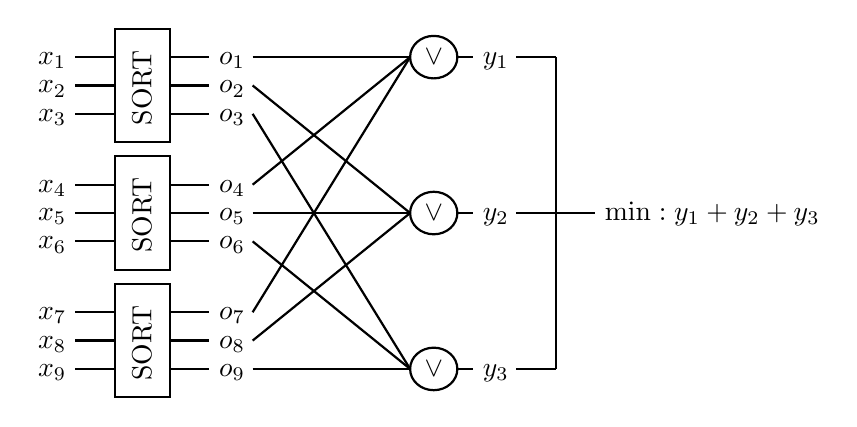
\begin{tikzpicture}[yscale=.9]
\draw[thick,-] (0,1.2) -- (-0.5,1.2);
\draw[thick,-] (0,0.8) -- (-0.5,0.8);
\draw[thick,-] (0,0.4) -- (-0.5,0.4);
\draw[] (-1.1,1.4) node[anchor=north west] {$x_1$};
\draw[] (-1.1,1) node[anchor=north west] {$x_2$};
\draw[] (-1.1,0.6) node[anchor=north west] {$x_3$};
\draw[thick,-] (0.7,1.2) -- (1.2,1.2);
\draw[thick,-] (0.7,0.8) -- (1.2,0.8);
\draw[thick,-] (0.7,0.4) -- (1.2,0.4);
\draw[] (1.2,1.4) node[anchor=north west] {$o_1$};
\draw[] (1.2,1) node[anchor=north west] {$o_2$};
\draw[] (1.2,0.6) node[anchor=north west] {$o_3$};
\draw[thick] (0,0) rectangle (0.7,1.6);
\draw[] (0.1,0.1) node[anchor=north west,rotate=90] {SORT};
\draw[thick,-] (0,-0.6) -- (-0.5,-0.6);
\draw[thick,-] (0,-1) -- (-0.5,-1);
\draw[thick,-] (0,-1.4) -- (-0.5,-1.4);
\draw[] (-1.1,-0.4) node[anchor=north west] {$x_4$};
\draw[] (-1.1,-0.8) node[anchor=north west] {$x_5$};
\draw[] (-1.1,-1.2) node[anchor=north west] {$x_6$};
\draw[thick,-] (0.7,-0.6) -- (1.2,-0.6);
\draw[thick,-] (0.7,-1) -- (1.2,-1);
\draw[thick,-] (0.7,-1.4) -- (1.2,-1.4);
\draw[] (1.2,-0.4) node[anchor=north west] {$o_4$};
\draw[] (1.2,-0.8) node[anchor=north west] {$o_5$};
\draw[] (1.2,-1.2) node[anchor=north west] {$o_6$};
\draw[thick] (0,-1.8) rectangle (0.7,-0.2);
\draw[] (0.1,-1.7) node[anchor=north west,rotate=90] {SORT};
\draw[thick,-] (0,-2.4) -- (-0.5,-2.4);
\draw[thick,-] (0,-2.8) -- (-0.5,-2.8);
\draw[thick,-] (0,-3.2) -- (-0.5,-3.2);
\draw[] (-1.1,-2.2) node[anchor=north west] {$x_7$};
\draw[] (-1.1,-2.6) node[anchor=north west] {$x_8$};
\draw[] (-1.1,-3) node[anchor=north west] {$x_9$};
\draw[thick,-] (0.7,-2.4) -- (1.2,-2.4);
\draw[thick,-] (0.7,-2.8) -- (1.2,-2.8);
\draw[thick,-] (0.7,-3.2) -- (1.2,-3.2);
\draw[] (1.2,-2.2) node[anchor=north west] {$o_7$};
\draw[] (1.2,-2.6) node[anchor=north west] {$o_8$};
\draw[] (1.2,-3) node[anchor=north west] {$o_9$};
\draw[thick] (0,-3.6) rectangle (0.7,-2);
\draw[] (0.1,-3.5) node[anchor=north west,rotate=90] {SORT};
\draw[thick,-] (1.75,1.2) -- (3.75,1.2); \draw[thick,-] (1.75,-0.6) -- (3.75,1.2); \draw[thick,-] (1.75,-2.4) -- (3.75,1.2); \draw[] (3.81,1.45) node[anchor=north west] {$\vee$};
\draw[thick] (4.05,1.2) circle (0.3);
\draw[thick,-] (4.35,1.2) -- (4.55,1.2);
\draw[thick,-] (5.1,1.2) -- (5.6,1.2);
\draw[] (4.55,1.4) node[anchor=north west] {$y_1$};
\draw[thick,-] (1.75,0.8) -- (3.75,-1); \draw[thick,-] (1.75,-1) -- (3.75,-1); \draw[thick,-] (1.75,-2.8) -- (3.75,-1); \draw[] (3.81,-0.75) node[anchor=north west] {$\vee$};
\draw[thick] (4.05,-1) circle (0.3);
\draw[thick,-] (4.35,-1) -- (4.55,-1);
\draw[thick,-] (5.1,-1) -- (5.6,-1);
\draw[] (4.55,-0.8) node[anchor=north west] {$y_2$};
\draw[thick,-] (1.75,0.4) -- (3.75,-3.2); \draw[thick,-] (1.75,-1.4) -- (3.75,-3.2); \draw[thick,-] (1.75,-3.2) -- (3.75,-3.2); \draw[] (3.81,-2.95) node[anchor=north west] {$\vee$};
\draw[thick] (4.05,-3.2) circle (0.3);
\draw[thick,-] (4.35,-3.2) -- (4.55,-3.2);
\draw[thick,-] (5.1,-3.2) -- (5.6,-3.2);
\draw[] (4.55,-3) node[anchor=north west] {$y_3$};
\draw[thick,-] (5.6,1.2) -- (5.6,-3.2);
\draw[thick,-] (5.6,-1) -- (6.1,-1);
\draw[] (6.1,-0.7) node[anchor=north west] {$\min:y_1+y_2+y_3$};
    \end{tikzpicture}
    \caption{Schematic depiction of the encoding of the $1^{\text{st}}$ iteration of the SAT-based algorithm.}
    \label{fig:algo-enc-1}
\end{figure} 
In the iterations where $i>1$, it is necessary to consider that some
objective functions are relaxed. Hence, for each objective function $f_j$, 
we add fresh Boolean variables $s^i_{1,j},\dots,s^i_{m_j,j}$, $j=1,\dots,n$.
In addition, we add to $\mathcal{H}$ clauses enforcing that if $r^i_j$ is false
(i.e.\ objective function $f_j$ is not relaxed when finding the $i$-th maximum), 
then $(s^i_{1,j},\dots,s^i_{m_j,j})$ is equal to $(o_{1,j},\dots,o_{m_j,j})$, for 
$j=1,\dots,n$.
Finally, instead of doing the componentwise disjunction between the outputs of the sorting networks, we do it between the new vectors $(s^i_{1,j},\dots,s^i_{m_j,j})$, $j=1,\dots,n$.
Note that the relaxation variables allows some of these vectors to assume 
arbitrary values. However, since we are minimising, those vectors can safely
be assigned to false and will not affect the componentwise disjunction.
As a result, the vector resulting from the componentwise disjunction, $(y^i_1,\dots,y^i_m)$, will correspond to the maximum of $n-i+1$ objective functions.
Figure~\ref{fig:algo-enc-2} illustrates the encoding used for the second iteration. The next iterations follow the same schema. 
Observe that the sorting networks do not have to be rebuilt between iterations.
The encoding of the objective function expressions using the sorting networks 
is done only once.

\begin{figure}[t]
\centering
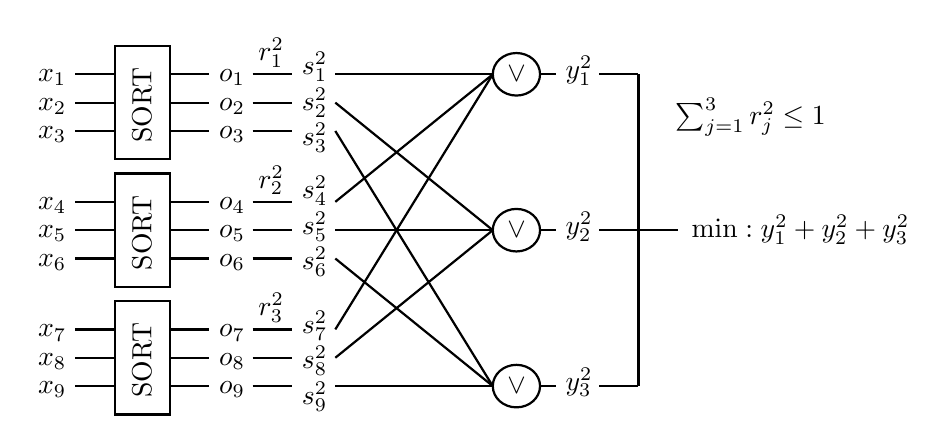
\begin{tikzpicture}[yscale=.9]
\draw[thick,-] (0,1.2) -- (-0.5,1.2);
\draw[thick,-] (0,0.8) -- (-0.5,0.8);
\draw[thick,-] (0,0.4) -- (-0.5,0.4);
\draw[] (-1.1,1.4) node[anchor=north west] {$x_1$};
\draw[] (-1.1,1) node[anchor=north west] {$x_2$};
\draw[] (-1.1,0.6) node[anchor=north west] {$x_3$};
\draw[thick,-] (0.7,1.2) -- (1.2,1.2);
\draw[thick,-] (0.7,0.8) -- (1.2,0.8);
\draw[thick,-] (0.7,0.4) -- (1.2,0.4);
\draw[] (1.2,1.4) node[anchor=north west] {$o_1$};
\draw[] (1.2,1) node[anchor=north west] {$o_2$};
\draw[] (1.2,0.6) node[anchor=north west] {$o_3$};
\draw[thick] (0,0) rectangle (0.7,1.6);
\draw[] (0.1,0.1) node[anchor=north west,rotate=90] {SORT};
\draw[thick,-] (0,-0.6) -- (-0.5,-0.6);
\draw[thick,-] (0,-1) -- (-0.5,-1);
\draw[thick,-] (0,-1.4) -- (-0.5,-1.4);
\draw[] (-1.1,-0.4) node[anchor=north west] {$x_4$};
\draw[] (-1.1,-0.8) node[anchor=north west] {$x_5$};
\draw[] (-1.1,-1.2) node[anchor=north west] {$x_6$};
\draw[thick,-] (0.7,-0.6) -- (1.2,-0.6);
\draw[thick,-] (0.7,-1) -- (1.2,-1);
\draw[thick,-] (0.7,-1.4) -- (1.2,-1.4);
\draw[] (1.2,-0.4) node[anchor=north west] {$o_4$};
\draw[] (1.2,-0.8) node[anchor=north west] {$o_5$};
\draw[] (1.2,-1.2) node[anchor=north west] {$o_6$};
\draw[thick] (0,-1.8) rectangle (0.7,-0.2);
\draw[] (0.1,-1.7) node[anchor=north west,rotate=90] {SORT};
\draw[thick,-] (0,-2.4) -- (-0.5,-2.4);
\draw[thick,-] (0,-2.8) -- (-0.5,-2.8);
\draw[thick,-] (0,-3.2) -- (-0.5,-3.2);
\draw[] (-1.1,-2.2) node[anchor=north west] {$x_7$};
\draw[] (-1.1,-2.6) node[anchor=north west] {$x_8$};
\draw[] (-1.1,-3) node[anchor=north west] {$x_9$};
\draw[thick,-] (0.7,-2.4) -- (1.2,-2.4);
\draw[thick,-] (0.7,-2.8) -- (1.2,-2.8);
\draw[thick,-] (0.7,-3.2) -- (1.2,-3.2);
\draw[] (1.2,-2.2) node[anchor=north west] {$o_7$};
\draw[] (1.2,-2.6) node[anchor=north west] {$o_8$};
\draw[] (1.2,-3) node[anchor=north west] {$o_9$};
\draw[thick] (0,-3.6) rectangle (0.7,-2);
\draw[] (0.1,-3.5) node[anchor=north west,rotate=90] {SORT};
\draw[thick,-] (1.75,1.2) -- (2.25,1.2);
\draw[thick,-] (1.75,0.8) -- (2.25,0.8);
\draw[thick,-] (1.75,0.4) -- (2.25,0.4);
\draw[] (2.25,1.65) node[anchor=north west] {$s^2_1$};
\draw[] (2.25,1.15) node[anchor=north west] {$s^2_2$};
\draw[] (2.25,0.65) node[anchor=north west] {$s^2_3$};
\draw[] (1.7,1.85) node[anchor=north west] {$r^2_1$};
\draw[thick,-] (1.75,-0.6) -- (2.25,-0.6);
\draw[thick,-] (1.75,-1) -- (2.25,-1);
\draw[thick,-] (1.75,-1.4) -- (2.25,-1.4);
\draw[] (2.25,-0.1) node[anchor=north west] {$s^2_4$};
\draw[] (2.25,-0.6) node[anchor=north west] {$s^2_5$};
\draw[] (2.25,-1.1) node[anchor=north west] {$s^2_6$};
\draw[] (1.7,0.05) node[anchor=north west] {$r^2_2$};
\draw[thick,-] (1.75,-2.4) -- (2.25,-2.4);
\draw[thick,-] (1.75,-2.8) -- (2.25,-2.8);
\draw[thick,-] (1.75,-3.2) -- (2.25,-3.2);
\draw[] (2.25,-2) node[anchor=north west] {$s^2_7$};
\draw[] (2.25,-2.5) node[anchor=north west] {$s^2_8$};
\draw[] (2.25,-3) node[anchor=north west] {$s^2_9$};
\draw[] (1.7,-1.75) node[anchor=north west] {$r^2_3$};
\draw[] (7,1) node[anchor=north west] {$\sum_{j=1}^3 r^2_j \leq 1$};
\draw[thick,-] (2.8,1.2) -- (4.8,1.2); \draw[thick,-] (2.8,-0.6) -- (4.8,1.2); \draw[thick,-] (2.8,-2.4) -- (4.8,1.2); \draw[] (4.86,1.45) node[anchor=north west] {$\vee$};
\draw[thick] (5.1,1.2) circle (0.3);
\draw[thick,-] (5.4,1.2) -- (5.6,1.2);
\draw[thick,-] (6.15,1.2) -- (6.65,1.2);
\draw[] (5.6,1.6) node[anchor=north west] {$y^2_1$};
\draw[thick,-] (2.8,0.8) -- (4.8,-1); \draw[thick,-] (2.8,-1) -- (4.8,-1); \draw[thick,-] (2.8,-2.8) -- (4.8,-1); \draw[] (4.86,-0.75) node[anchor=north west] {$\vee$};
\draw[thick] (5.1,-1) circle (0.3);
\draw[thick,-] (5.4,-1) -- (5.6,-1);
\draw[thick,-] (6.15,-1) -- (6.65,-1);
\draw[] (5.6,-0.6) node[anchor=north west] {$y^2_2$};
\draw[thick,-] (2.8,0.4) -- (4.8,-3.2); \draw[thick,-] (2.8,-1.4) -- (4.8,-3.2); \draw[thick,-] (2.8,-3.2) -- (4.8,-3.2); \draw[] (4.86,-2.95) node[anchor=north west] {$\vee$};
\draw[thick] (5.1,-3.2) circle (0.3);
\draw[thick,-] (5.4,-3.2) -- (5.6,-3.2);
\draw[thick,-] (6.15,-3.2) -- (6.65,-3.2);
\draw[] (5.6,-2.8) node[anchor=north west] {$y^2_3$};
\draw[thick,-] (6.65,1.2) -- (6.65,-3.2);
\draw[thick,-] (6.65,-1) -- (7.15,-1);
\draw[] (7.2,-0.65) node[anchor=north west] {$\min:y^2_1+y^2_2+y^2_3$};
    \end{tikzpicture}
    \caption{Schematic depiction of the encoding of the $2^{\text{nd}}$ iteration of the SAT-based algorithm.}
\label{fig:algo-enc-2}
\end{figure} 
\subsection{Core-guided Algorithm}
\label{sec:corePB}

In this section, we present the structure of our core-guided algorithm for 
leximax Boolean optimisation. The main goal of the core-guided algorithm is 
to only consider a subset of the variables in each objective function, thus
improving the performance of each call. 

Given a CNF formula $\varphi$, we assume that a call to a SAT solver to check
the satisfiability of $\varphi$ returns a triple $(st, \alpha, \mathcal{C})$,
where $st$ is a Boolean that is true if and only if $\varphi$ is satisfiable.
If $\varphi$ is satisfiable, then $\alpha$ contains a satisfying assignment.
Otherwise, if $\varphi$ is unsatisfiable, then $\mathcal{C}$ contains 
an unsatisfiable subformula (also known as an unsatisfiable core) of $\varphi$.

\begin{algorithm}[t]
\DontPrintSemicolon
\KwIn{A set of hard constraints $\mathcal{H}$ and objective functions $f_1,\dots,f_n$.}
\KwOut{A leximax-optimal solution $\alpha$.}
$\mathcal{X}\gets \bigcup_{j=1}^n \{\neg x : x\in f_j \}$\;
\For{$i \gets 1$ \KwTo $n$}{
    $\mathcal{H}\gets \mathcal{H}\cup \left\{\sum_{j=1}^n r^i_j \leq i - 1\right\}$\;
    $\LB \gets 0$\; \label{alg:initLB}
    \Repeat{$st$}
    {
        $(st,\alpha,\mathcal{C})\gets \texttt{SAT}(\mathcal{H}\cup \left\{ \left( \texttt{EncodeCNF}(f_j \leq \LB) \vee r^i_j \right) : j =1,\dots,n\right\}\cup \mathcal{X})$\; \label{alg:PB-call}
        \If{$st$ = {\tt False}}{
            \lIf{$\mathcal{C}\cap \mathcal{X} = \emptyset$}{ 
                $\LB \gets \LB + 1$ \label{alg:increaseLB}
            }
            \lElse{
                $\mathcal{X} \gets \mathcal{X} \setminus \mathcal{C}$ \label{alg:removeCore}
            }
        }
    }
    $\mathcal{H}\gets \mathcal{H}\cup \{ \left( \texttt{EncodeCNF}(f_j \leq \LB) \vee  r^i_j \right) : j =1,\dots,n\}$\; \label{alg:fixLB}
}
\Return{$\alpha$}\;
\caption{Core-guided leximax optimisation algorithm.}
\label{algo:pb-core-guided}
\end{algorithm}

Algorithm~\ref{algo:pb-core-guided} shows the pseudocode of the core-guided algorithm.
First, we define a set $\mathcal{X}$ with unit clauses that are the
negation of the variables in all objective functions $f_1,\dots,f_n$.
As in Algorithm~\ref{algo:ILP}, we iterate over the number of objective functions
and in each iteration we find the smallest $i$-th maximum considering $n-i+1$
objective functions.
The main difference between Algorithm~\ref{algo:ILP} and Algorithm~\ref{algo:pb-core-guided} is that, in each iteration, 
we perform an UNSAT-SAT search procedure on the value of the $i$-th maximum
initially assuming all variables in the objective functions are false, 
i.e.\ initially all are set to the optimum value.
For finding the minimum $i$-th maximum, we start with a lower bound $\LB$ of 0 (line~\ref{alg:initLB}). Then, a SAT call bounds the value of
the non-relaxed objective functions to $\LB$. If the formula in line~\ref{alg:PB-call} is unsatisfiable and it does not depend on the
assumed values in $\mathcal{X}$, then we can safely increase the lower bound
(line~\ref{alg:increaseLB}). Otherwise, we remove from $\mathcal{X}$ the unit clauses that appear in the unsatisfiable core $\mathcal{C}$ (line~\ref{alg:removeCore}).
At the end of iteration $i$, the variable $\LB$ contains the smallest possible value for the $i$-maximum of the objective functions. Hence, we can fix this value (line~\ref{alg:fixLB}).

\subsection{SAT-based Core-guided Algorithm with Sorting Networks}
\label{sec:coreSAT}

Algorithm~\ref{algo:pb-core-guided} can be implemented using different CNF encodings for bounding the objective functions (lines~\ref{alg:PB-call} and~\ref{alg:fixLB}). In this section, we detail Algorithm~\ref{algo:pb-core-guided} using the sorting networks representation proposed in Section~\ref{sec:itersat}.

Note that in the core-guided algorithm proposed in Algorithm~\ref{algo:pb-core-guided}, the CNF encoding of PB constraints that bound the objective functions is simplified due to the unit clauses in the set $\mathcal{X}$ that fix the values of some variables. In developing this algorithm, the same technique using sorting networks from Section~\ref{sec:itersat} can be used to encode the objective functions, and use the set $\mathcal{X}$ to unit propagate the fixed values from the input of the sorting networks to the output.
However, we propose to improve on this. Instead of representing the entire objective functions in the beginning of the algorithm, we propose to construct sorting networks only for the objective variables that are not negated in $\mathcal{X}$. As a result, the sorting networks are built dynamically and incrementally. At first, the sorting networks are empty and grow as more variables from the objective functions are removed from $\mathcal{X}$ due to the unsatisfiable cores found during the SAT calls.

Using dynamic sorting networks raises some challenges. There are two main options for growing the sorting networks: (1)~build a new sorting network from scratch or (2)~grow the previous sorting network incrementally. 
However, the first case of rebuilding the sorting network might result in losing incremental SAT solving between iterations. An alternative would be to add a new blocking variable to the entire encoding of a sorting network and control if a given sorting network is active or not using the blocking variable and SAT solver assumptions.
Nevertheless, this last alternative still implies rebuilding the sorting networks and the size of the SAT formula might become too large to handle efficiently.
Due to these drawbacks, we propose to reuse the sorting network and make it grow in an incremental fashion. The incremental encoding to CNF has been the subject of previous research work~\cite{DBLP:journals/jsat/EenS06,DBLP:conf/cp/MartinsJML14} but it is new in the context of leximax optimisation.

Consider there is a sorting network that encodes some objective function and a new set of variables is to be added. In that case, we can build a sorting network for the new variables and apply a merge encoding between both sorting networks.
Figure~\ref{fig:merge-general-idea} illustrates the proposed schema for growing a sorting network where the Batcher's odd-even merge construction~\cite{batcher,knuth1997art} can be used.

\begin{figure}[t]
    \centering
    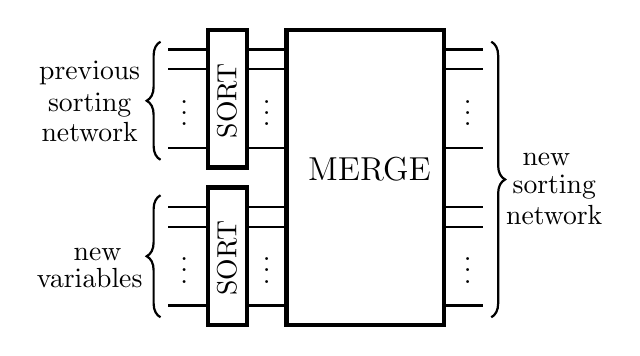
\begin{tikzpicture}
\draw[thick] (0,7) -- (0.5,7);
\draw[thick] (0,6.75) -- (0.5,6.75);
\draw[thick] (0,5.75) -- (0.5,5.75);
\draw[thick] (1,7) -- (1.5,7);
\draw[thick] (1,6.75) -- (1.5,6.75);
\draw[thick] (1,5.75) -- (1.5,5.75);
\draw[thick] (3.5,7) -- (4,7);
\draw[thick] (3.5,6.75) -- (4,6.75);
\draw[thick] (3.5,5.75) -- (4,5.75);
\draw[] (0.5,5.75) node[anchor=north west,rotate=90] {SORT};
\node at (0.2,6.3) {$\vdots$};
\node at (1.25,6.3) {$\vdots$};
\node at (3.8,6.3) {$\vdots$};
\draw[ultra thick] (0.5,5.5) rectangle (1,7.25);
\draw[thick] (0,5) -- (0.5,5);
\draw[thick] (0,4.75) -- (0.5,4.75);
\draw[thick] (0,3.75) -- (0.5,3.75);
\draw[thick] (1,5) -- (1.5,5);
\draw[thick] (1,4.75) -- (1.5,4.75);
\draw[thick] (1,3.75) -- (1.5,3.75);
\draw[thick] (3.5,5) -- (4,5);
\draw[thick] (3.5,4.75) -- (4,4.75);
\draw[thick] (3.5,3.75) -- (4,3.75);
\draw[] (0.5,3.75) node[anchor=north west,rotate=90] {SORT};
\node at (0.2,4.3) {$\vdots$};
\node at (1.25,4.3) {$\vdots$};
\node at (3.8,4.3) {$\vdots$};
\draw[ultra thick] (0.5,3.5) rectangle (1,5.25);
\draw[ultra thick] (1.5,3.5) rectangle (3.5,7.25);
\draw[] (1.65,5.75) node[anchor=north west] {\large MERGE};
\draw [decorate, thick,
    decoration = {brace, amplitude=5pt}] (-0.1,3.6) --  (-0.1,5.15);
\node at (-0.9,4.4) {new};
\node at (-1,4.1) {variables};
\draw [decorate, thick,
    decoration = {brace, amplitude=5pt}] (-0.1,5.6) --  (-0.1,7.1);
\node at (-1,6.7) {previous};
\node at (-1,6.3) {sorting};
\node at (-1,5.95) {network};
\draw [decorate, thick,
    decoration = {brace,mirror, amplitude=5pt}] (4.1,3.6) --  (4.1,7.1);
\node at (4.8,5.6) {new};
\node at (4.9,5.25) {sorting};
\node at (4.9,4.9) {network};
    \end{tikzpicture}
    \caption{General schema of growing a sorting network using sort and merge.}
    \label{fig:merge-general-idea}
\end{figure}

A sorting network with $k$ inputs with Batcher's odd-even merge sorting network uses $\Theta(k(\log(k))^2)$ comparators.
There are no known constructions that produce sorting networks with smaller size complexity that can be used in practice.
Thus, a sorting network with $k$ inputs is encoded with $\Omega(k(\log(k))^2)$ clauses.

There are situations where the proposed sort-and-merge approach may lead to a larger growth of the number of comparators (and thus the number of clauses) than expected. 
The issue is that if, each time we obtain a new unsatisfiable core, we remove the variables from $\mathcal{X}$ and add them straight away to the sorting networks, the number of comparators may grow with $k^2$, instead of $k(\log(k))^2$.
The odd-even merge construction produces $\Theta(k\log(k))$ comparators when merging two sequences of size $k$, and produces $\Theta(k)$ comparators when merging two sequences with size $k$ and $1$.
Therefore, the odd-even merge sorting network, which works by recursively sorting two subsequences and then merging them, only produces $\Theta(k(\log(k))^2)$ comparators when, in each recursive step, the sequence is cut in half.
However, if we have the scenario of merging a sequence of $k-1$ elements and a sequence of $1$ element, the final sorting network will contain $\Theta(k^2)$ comparators.
In the core-guided algorithm proposed in Algorithm~\ref{algo:pb-core-guided}, in the worst case, the unsatisfiable cores contain exactly one of the clauses in $\mathcal{X}$. As a result, it is possible to end up with sorting networks with $k$ inputs having $\Theta(k^2)$ comparators.

In order to try to limit the worst-case scenario where the encoding of the objective functions becomes quadratic, we propose to delay the merge process between the previous sorting network and the new variables to be added.
Hence, when an unsatisfiable core is identified in the SAT call (line~\ref{alg:PB-call} of Algorithm~\ref{algo:pb-core-guided}), we remove from $\mathcal{X}$ the clauses in the core, but the respective variables are not immediately added to the sorting networks.
Instead, the variables from the clauses in the unsatisfiable core are added to a set $\mathcal{S}$. 
Next, the SAT solver is repeatedly called with a smaller set $\mathcal{X}$ of unit clauses. For each new unsatisfiable core $\mathcal{C}$, clauses from $\mathcal{C} \cap \mathcal{X}$ are removed from $\mathcal{X}$ and their respective variables are added to $\mathcal{S}$.
When the SAT call becomes satisfiable, then we add the variables in $\mathcal{S}$ to the sorting networks and the set $\mathcal{S}$ is emptied.

This procedure consists in finding as many cores as possible of a formula that are disjoint with regard to $\mathcal{X}$. From now on, we refer to this strategy as the \emph{disjoint cores strategy}.
The use of disjoint cores is another idea borrowed from the MaxSAT solving literature~\cite{DBLP:conf/cp/DaviesB11,DBLP:conf/cp/BergJ17}.
Note that this option may reduce the number of times the sorting networks are extended during the algorithm's execution.
When extending the sorting networks by sort-and-merge, the disjoint cores strategy can prevent the worst case quadratic growth of the number of comparators. 

\begin{example}\label{eg:disjoint}
This example focuses solely on the delay of including literals from unsatisfiable cores into the sorting network representation of the objective functions.

Consider a MOBO instance with hard clauses $\mathcal{H}$ and two objective functions:
\begin{equation*}
    f_1 = x_1 + x_2 + x_3 + x_4; \quad f_2 = x_5 + x_6 + x_7 + x_8.
\end{equation*}
Assume at some point in the execution of the core-guided algorithm with dynamic sorting networks $\{x_1,x_2\}$ and $\{x_5,x_6\}$ are in the sorting networks and $\mathcal{X}=\{\neg x_3,\neg x_4,\neg x_7,\neg x_8\}$.
Suppose we are minimising $\max(f_1,f_2)$ and the lower bound is currently $1$.
The next call to the SAT solver is testing if there exists a feasible solution 
for the following formula:
\begin{equation}
    \mathcal{H} \quad \wedge \quad \bigwedge_{l \in \mathcal{X}} l \quad \wedge \quad x_1 + x_2 \leq 1 \quad \wedge \quad x_5 + x_6 \leq 1.\label{eq:disjoint-cores}
\end{equation}
Assume the formula is unsatisfiable and the core $\mathcal{C}$ is such that $\mathcal{C}\cap \mathcal{X}=\{\neg x_3\}$.
In this case, $\mathcal{X}$ is updated to $\{\neg x_4,\neg x_7,\neg x_8\}$.
There are two options.
The first option is to add $x_3$ to the sorting network of $f_1$ and continue with the algorithm by calling the SAT solver on the formula
\begin{equation}
    \mathcal{H} \quad \wedge \quad \bigwedge_{l \in \mathcal{X}} l \quad \wedge \quad x_1 + x_2 + x_3 \leq 1 \quad \wedge \quad x_5 + x_6 \leq 1.\label{eq:disjoint-cores2}
\end{equation}
However, as previously explained, this option may lead to an undesirable growth of the number of clauses in the objective function CNF representation.
Hence, using the disjoint cores strategy, $x_3$ is not added to the sorting network right away.
Instead we store $x_3$ in a set $\mathcal{S}$, but we still remove $\neg x_3$ from $\mathcal{X}$.
Then, we test once again if~(\ref{eq:disjoint-cores}) is true, but now $x_3$ can be true because it is no longer in $\mathcal{X}$.

Assume the formula is still unsatisfiable and the new unsatisfiable core $\mathcal{C}$ is such that $\mathcal{C}\cap\mathcal{X}=\{\neg x_7\}$.
We remove $\neg x_7$ from $\mathcal{X}$ and add $x_7$ to $\mathcal{S}$, so now $\mathcal{S}=\{x_3,x_7\}$ and $\mathcal{X} = \{\neg x_4,\neg x_8\}$.
We check again the formula (\ref{eq:disjoint-cores}) where $x_7$ can now be true.
Assume the formula is still unsatisfiable and the new core $\mathcal{C}$ is such that $\mathcal{C}\cap\mathcal{X}=\{\neg x_4\}$.
Then, $\neg x_4$ is removed from $\mathcal{X}$ and $x_4$ is added to $\mathcal{S}$.
Assume that (\ref{eq:disjoint-cores}) becomes satisfiable.
Notice that this does not mean the optimal solution has been found, as $\max(f_1,f_2)$ may not be $1$ for the feasible solution.
We need to add the variables in $\mathcal{S}$ to the sorting networks and then check if there exists a feasible solution such that
\begin{equation}
    \mathcal{H} \quad \wedge \quad \bigwedge_{l \in \mathcal{X}} l \quad \wedge \quad x_1 + x_2 + x_3 + x_4 \leq 1 \quad \wedge \quad x_5 + x_6 + x_7 \leq 1,\label{eq:disjoint-cores3}
\end{equation}
with $\mathcal{X} = \{\neg x_8\}$.
If the formula (\ref{eq:disjoint-cores3}) is unsatisfiable, we repeat the previous steps of removing literals from $\mathcal{X}$ (in this case only $\neg x_8$ is left) until the formula becomes satisfiable.
\end{example}  
\section{Evaluation}
\label{sec:evaluation}

This section evaluates the proposed SAT-based algorithms for leximax optimisation. Besides comparing the different strategies of our algorithms, we compare against the state of the art ILP-based approach.
The algorithms based on Constraint Programming~\cite{bouveret2009computing} are not included since we were unable to find a publicly available implementation.

\subsection{Use Case: Package Upgradeability}

The Package Upgradeability problem is an NP-complete problem~\cite{DiCosmo2006-NP} that arises when a user of a software system (e.g.\ Linux distributions) wants to install, remove or upgrade software packages. In the final installation, for each package $p_i$ that is installed, all its dependencies must be satisfied and there cannot be any other installed package $p_j$ such that $p_i$ and $p_j$ are conflicting.
In addition, the user can define several objective functions to be minimised, such as the number of newly installed packages, the number of removed packages, or the number of not up-to-date packages. Therefore, the Package Upgradeability problem can be modelled as a MOBO formula.
Furthermore, it is often the case that the user is unable to define a proper order of preferences among the several objectives. Hence, our evaluation is focused on finding a leximax-optimal solution for the Package Upgradeability problem.

There are several Package Upgradeability solvers that rely on encodings to Answer Set Programming~\cite{aspcud}, Maximum Satisfiability~\cite{Janota2012,Janota2014}, Pseudo-Boolean Optimisation~\cite{inesc-and-p2cudf} and ILP~\cite{milp2010, mancoosi-del-4.3}.
However, most tools only compute lexicographically optimal solutions of the problem. Only \texttt{mccs}~\cite{mccs-webpage,milp2010} (version 1.1) is able to compute leximax-optimal solutions, using the ILP-based algorithm described in Algorithm~\ref{algo:ILP}.
\texttt{mccs} can be used with different ILP solvers. Hence, we configured and tested \texttt{mccs} with the following ILP solvers: \texttt{CPLEX}~\cite{cplex-webpage} (version 12.10.0), \texttt{Gurobi}~\cite{gurobi-webpage} (version 9.0.3), \texttt{SCIP}~\cite{scip,scip-webpage} (version 7.0.1), \texttt{Cbc}~\cite{cbc-webpage} (version devel, build Jan 14 2021), \texttt{GLPK}~\cite{glpk-webpage} (version 4.65) and \texttt{lpsolve}~\cite{lpsolve-webpage} (version 5.5.2.5).

\subsection{Implementation and Benchmarks}

The new SAT-based algorithms and the existing ILP-based algorithm were implemented in a tool for leximax optimisation that is publicly available~\cite{leximaxIST}. 
In the implementation of the SAT-based algorithms, the Batcher's odd–even merge procedure~\cite{batcher,knuth1997art} was used for constructing and merging sorting networks.
The sorting network encoding of \textsc{MiniSat+}~\cite{DBLP:journals/jsat/EenS06} was used  without coefficient decomposition and interconnected sorting networks since we focus on solving unweighted instances (e.g. Package Upgradeability).
To evaluate the SAT-based algorithms on the Package Upgradeability domain, the \texttt{packup}~\cite{Janota2012,Janota2014,packup-webpage} Package Upgradeability solver was linked with our tool.
The algorithms were evaluated using the incremental SAT solving library of \texttt{CaDiCaL}~\cite{cadical} (version 1.3.1).

The Package Upgradeability solvers, \texttt{packup} and \texttt{mccs}, were executed on a set of 142 Package Upgradeability benchmarks~\cite{benchmarks_packup} from the Mancoosi International Solver Competition~\cite{mancoosi-competition}.
The objective functions defined in the Mancoosi competition are the following: \textit{removed}, \textit{notuptodate}, \textit{changed}, \textit{unsat\_recommends} and \textit{new}.
For each of the 142 benchmarks we generated instances considering all 26 combinations of two, three, four and five objective functions, resulting in 3692 instances.
Of the 3692 instances, 122 instances correspond to unsatisfiable instances or instances that are reduced to the single-objective case. As a result, the final benchmark set contains 3570 instances to find a leximax-optimal solution.

In order to broaden the experimental evaluation, we adapted a subset of benchmark instances from the MaxSAT Evaluation 2021~\cite{maxsat-eval-2021} to the multi-objective domain.
From the 561 benchmarks of the unweighted track of the MaxSAT Evaluation 2021, we selected 100 instances that encode problems from different domains, such that the MaxSAT solver \texttt{Open-WBO}~\cite{open-wbo, open-wbo-webpage} outperforms \texttt{Gurobi} within a 10~s timeout.
For each of those benchmarks, a MOBO instance was generated by keeping the same set of constraints and by randomly partitioning the original set of soft clauses into multiple sets of soft clauses.
We considered partitions into two, three and four objective functions, resulting in a set of 300 instances~\cite{mse21_pbmo_benchmarks}. 

All algorithms were executed on a single thread, with 180 seconds CPU time limit for the Package Upgradeability instances and 3600 seconds CPU time limit in the case of MaxSAT-based instances. 
The experiments were run on Intel(R) Xeon(R) E5-2630 v2 CPU 2.60GHz machines with Debian Linux operating system with 4~GB memory limit for each instance.

\subsection{Evaluation of the SAT-based Algorithms}

This section analyses the performance of the different versions of the proposed SAT-based algorithms on the set of Package Upgradeability benchmarks.

First we describe the abbreviations used when presenting the results for these versions.
There are three versions of Algorithm~\ref{algo:ILP} using the SAT encoding as described in Section~\ref{sec:itersat}, each corresponding to different types of search for the $i$-th maximum: the linear search SAT-UNSAT algorithm is \texttt{linear-su}, linear search UNSAT-SAT is \texttt{linear-us} and binary search is \texttt{binary}.
There are several versions of the core-guided algorithm proposed in Section~\ref{sec:coreSAT}.
The version where the sorting networks are rebuilt with non-incremental SAT solving is named \texttt{core-rebuild}. If the sorting networks are rebuilt, but using incremental SAT solving then we use \texttt{core-rebuild-incr}.
If the objective functions are statically built at the beginning of the algorithm we use \texttt{core-static}.
The version with dynamic sorting networks that extends the objective functions by sorting the new variables and merging with the previous sorting network is \texttt{core-merge}.
If the additional disjoint cores strategy is used, then the algorithms' names are appended with `\texttt{-dc}'.

\begin{figure}[t]
  \begin{centering}
    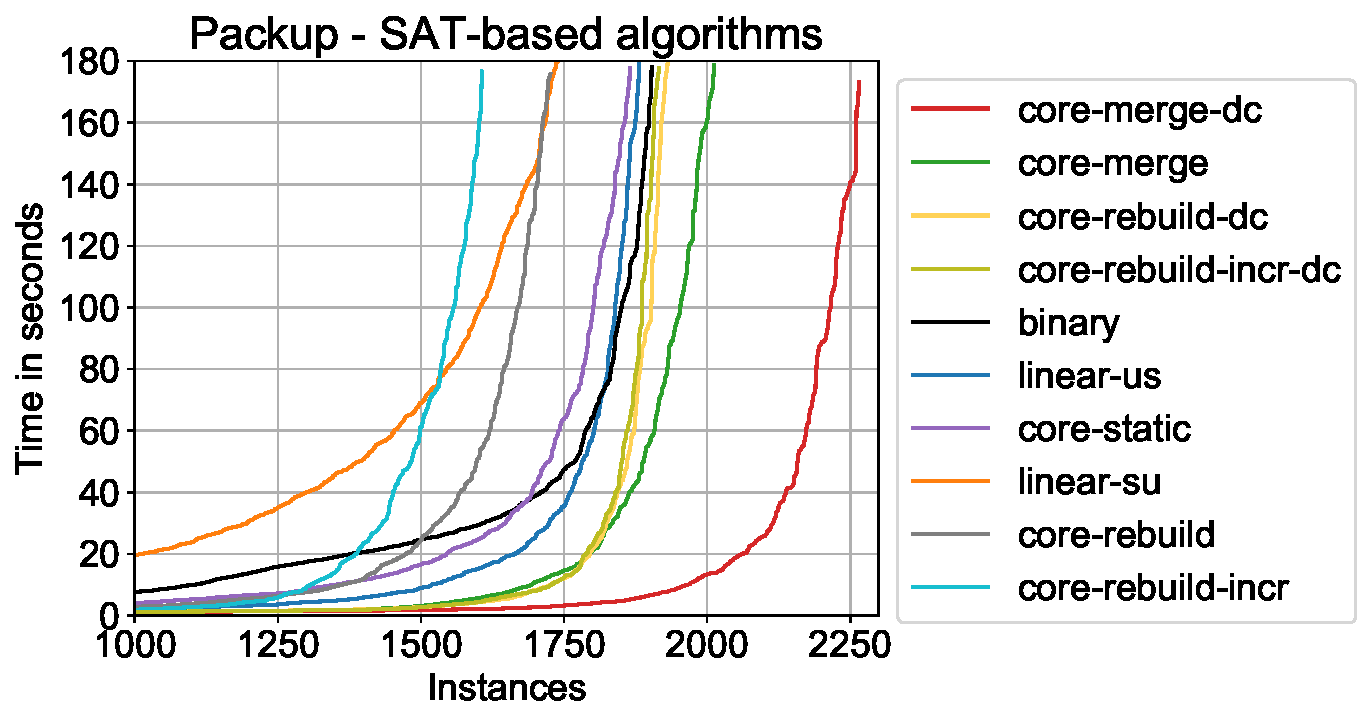
\includegraphics[width=0.75\textwidth]{images/package_upgradeability/run_times_packup.pdf}
    \caption{Run times of SAT-based algorithms on Package Upgradeability instances (180 seconds).}
    \label{fig:run-times-packup}
  \end{centering}
\end{figure}

Figure~\ref{fig:run-times-packup} shows a cactus plot with the run times of solved Package Upgradeability instances by SAT-based algorithms.
Among the different versions of the iterative SAT-based algorithm, the best performing was the binary search. Nevertheless, despite being able to solve more instances within the time limit of 180 seconds, it is usually slower than the UNSAT-SAT search when this approach is able to solve the instance. For example, the plot clearly shows that the number of instances solved by the binary search within 20 seconds is much smaller.

The results from Figure~\ref{fig:run-times-packup} also show that the core-guided approach using the proposed incremental merge of sorting networks is the best performing algorithm. Moreover, delaying the merge operation by using the disjoint cores strategy results in a significant performance boost. Observe that the disjoint cores strategy also greatly improves the algorithms that rebuild the sorting networks (both the incremental and non-incremental versions). 

\begin{figure}[t]
  \centering
  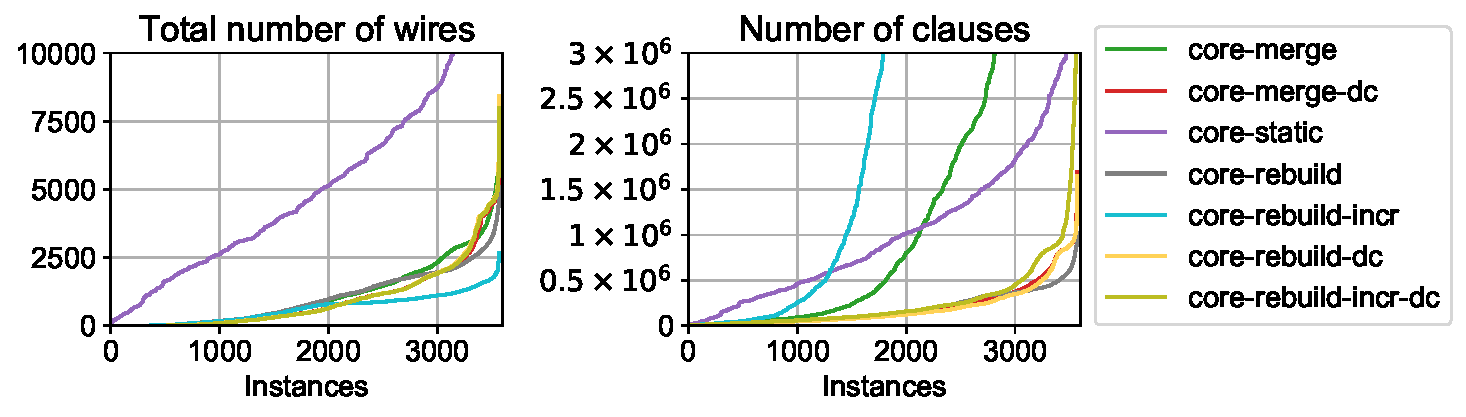
\includegraphics[width=1\linewidth]{images/package_upgradeability/snet_info.pdf}
  \caption{Cactus plots of the sum of the number of wires of the sorting networks (on the left) and the number of clauses (on the right) at the time of the last SAT call.}
  \label{fig:wires_clauses}
\end{figure}

To better understand the difference in the performance of the algorithms, we analyse the number of wires of the sorting networks and the number of clauses of the formula.
Figure~\ref{fig:wires_clauses} contains two cactus plots. Both plots correspond to the Package Upgradeability benchmarks. The plot on the left shows the total number of wires of the last sorting networks produced by each algorithm. The plot on the right shows the number of clauses of the last call to the SAT solver.
As expected, using dynamic sorting networks allows to significantly reduce the number of wires of the sorting networks when compared with the static representation of the objective functions. This occurs because not all variables are represented in the objective functions.
The goal is that the reduction in the number of wires allows a reduction in the number of comparators and ultimately in the number of clauses.
Indeed, we observe a significant reduction in the number of clauses with dynamic sorting networks, except for \texttt{core-rebuild-incr}, because it does not delete the previous sorting network encodings, and \texttt{core-merge}, because of the growth of the number of comparators when merging.
Since there are many small unsatisfiable cores, the growth in \texttt{core-merge} tends to approximate the worst case scenario explained in Section~\ref{sec:coreSAT}.
Due to this growth on the size of the formula, \texttt{core-rebuild-incr} and \texttt{core-merge} exceeded the 4~GB memory limit in around $30\%$ and $4\%$ of the instances, respectively.
The right plot of Figure~\ref{fig:wires_clauses} clearly shows the impact of using the disjoint cores strategy, resulting in a significant reduction in the size of the final sorting networks. 
Note that \texttt{core-merge-dc} and \texttt{core-rebuild-incr-dc} both use incremental SAT solving, and produce a similar number of clauses.
However, the sort-and-merge approach proved to be more effective than the rebuild approach, as \texttt{core-merge-dc} solved more instances with overall faster run times than \texttt{core-rebuild-incr-dc}.

\subsection{Comparison with ILP solvers}
\label{sec:eval-comp-ilp}
This section provides a comparison between the best performing core-guided SAT approach \texttt{core-merge-dc} and the iterative ILP algorithm when using different ILP solvers.

\begin{figure}[t]
  \centering
  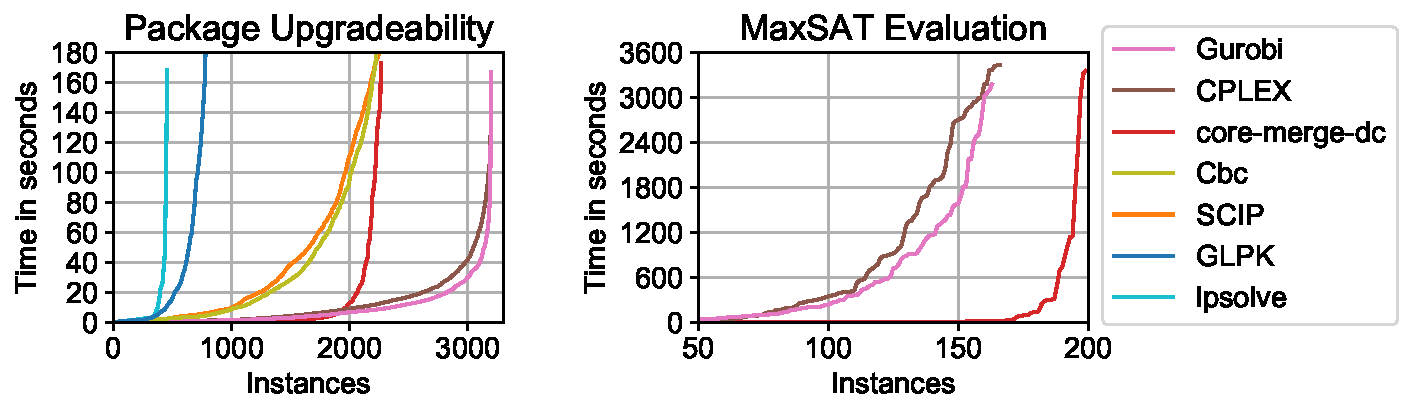
\includegraphics[width=1\linewidth]{images/pack_mse21_join.pdf}
  \caption{Run times of solved instances on Package Upgradeability benchmarks (left) and generated multi-objective instances based on the MaxSAT Evaluation 2021 (right).}
  \label{fig:run-times-global}
\end{figure}

Figure~\ref{fig:run-times-global} shows the cactus plots of the run times of solved instances, for each solver.
On the left we the results for the Package Upgradeability benchmarks and on the right the results on the instances generated from the MaxSAT Evaluation 2021.

In the case of Package Upgradeability, the overall results show that when using commercial solvers \texttt{Gurobi} and \texttt{CPLEX}, the iterative ILP approach solves more instances. However, the plot also shows that our approach can outperform the iterative ILP algorithm when using non-commercial solvers in both the number of instances and run-times. We note that in many real-world cases, such as the Package Upgradeability problem in open-source Linux distributions, the usage of commercial solvers is not feasible.

On the MaxSAT Evaluation 2021 instances, we tested the ILP approach using commercial solvers \texttt{Gurobi} and \texttt{CPLEX}.
These results suggest that our proposed algorithm can potentially outperform the ILP commercial solvers in other application domains, e.g.\ the Placement Fixer problem, which is not well-suited for ILP, because of the type of constraints~\cite{DBLP:conf/tacas/NadelR16}.

\begin{figure}[t]
  \centering
  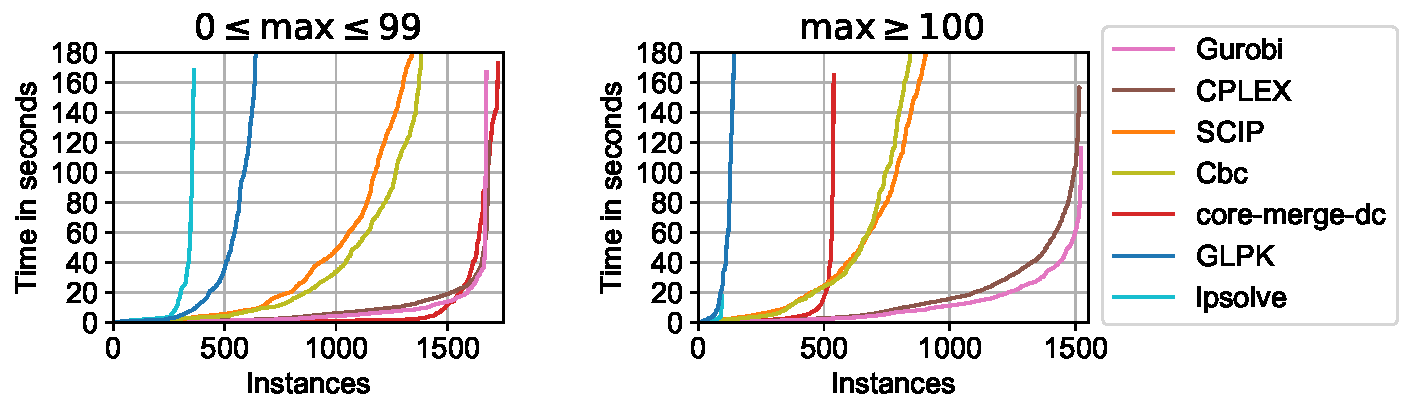
\includegraphics[width=1\linewidth]{images/package_upgradeability/by_opt_val.pdf}
  \caption{Run times of \texttt{core-merge-dc} and the ILP solvers on Package Upgradeability benchmarks, with an optimal maximum of the objective vector $\leq 99$ on the left and $\geq 100$ on the right.}
  \label{fig:run-times-by-opt-val}
 \end{figure}

Figure~\ref{fig:run-times-by-opt-val} shows two cactus plots that provide an analysis on the algorithms' performance depending on the values in the leximax-optimal objective vector in the Package Upgradeability instances.
The plot on the left shows the run times for instances where the largest value in the leximax-optimal solution is smaller than 100.
On the other hand, the plot on the right shows the run times for instances where the largest value is larger than or equal to 100.

Observe that when the largest value is smaller than $100$, \texttt{core-merge-dc} has a similar performance to the iterative ILP algorithm when using commercial solvers \texttt{CPLEX} or \texttt{Gurobi} and clearly outperforms non-commercial solvers.
On the other hand, the iterative ILP algorithm has a stronger performance for larger values in the leximax-optimal solution.
This occurs since our core-guided approach is slower to converge in these situations~\cite{detailed-tables}.
Nevertheless, in the context of package upgradeability, it is often the case that real-world users perform incremental adjustments to a current installation. Hence, in these situations, optimal solutions tend to have a small cardinality and our proposed \texttt{core-merge-dc} algorithm excels in those scenarios. 
\section{Conclusions}
\label{sec:concl}

This paper introduces the first SAT-based leximax optimisation algorithms.
Besides iterative SAT-based algorithms, we also propose a new core-guided algorithm for leximax optimisation. The algorithms are built upon the effective encoding of PB constraints to CNF and a CNF encoding to determine the maximum value among several objective functions.
Moreover, we explore the translation of PB constraints to CNF using sorting networks. We use a merging technique that allows to dynamically and incrementally extend the representation of objective functions. Additionally, a strategy based on the identification of disjoint cores in the core-guided algorithm allows to delay the merging process, thus resulting in a more effective encoding of the objective functions.

An experimental evaluation is carried out on the Multi-Objective Package Upgradeability Optimisation problem and on generated MOBO instances based on the MaxSAT Evaluation benchmarks.
The core-guided algorithm outperforms the iterative ILP algorithm when using non-commercial solvers on the Package Upgradeability benchmarks.
The results on the MaxSAT Evaluation instances suggest that our SAT-based algorithms may be competitive with the ILP algorithm with commercial solvers on other application domains.

As a future direction of research, we highlight the integration of our leximax optimisation algorithms with incomplete algorithms, such as \texttt{Polosat}~\cite{DBLP:conf/fmcad/Nadel20a}, in the same way they are currently integrated to MaxSAT solvers.
Another interesting direction of research is the development of hybrid approaches using SAT and ILP solvers for leximax optimisation, e.g.\ by adapting the approach of the MaxSAT solver \texttt{MaxHS}~\cite{DBLP:conf/cp/DaviesB11}.
 
\bibliography{refs}
\end{document}
